\chapter{Détecteurs de neutrons}
\section{Principes de la détection neutrons}
Étant des particules non-chargées, les neutrons ne peuvent pas être directement détectés. Ils se
détectent essentiellement par leurs interactions avec des noyaux atomiques via des réactions
nucléaires donnant naissance à des particules chargées détectables (proton, $\alpha$, fragments de
fission, \dots).\\

Les section efficaces des neutrons sont très dépendantes de l'énergie du neutron, au point qu'on 
considère deux domaines d'énergies: lents ($E<0.5$ eV) et rapide ($E>0.5$ eV).

\subsection{Matériaux utilisés pour la détection des neutrons}%sl5
Forcément, la section efficace d'interaction doit être grande afin de ne pas avoir un détecteur
énorme. De plus, le champ de neutron est souvent accompagné d'un champ (intense) de $\gamma$ qu'il
faudra éventuellement discriminer. La valeur de $Q$ (énergie libérée) prendra alors tout son sens. 
Plus elle augmente, plus l'énergie cédée aux produits de fission augmente et plus il sera facile de
discriminer les $\gamma$. La distances parcourue par les produits de réaction a aussi de l'importance.

\subsubsection{Réactions importantes pour la détection de neutrons} 
Ce genre de réaction important est à connaître ($Q\approx3$). Une connue est celle du 
$^{10}$B(n,$\alpha$)
\begin{equation}
^{10}_5B+^1_0n \rightarrow \left\{
\begin{aligned}
   &^7_3Li+^4_2\alpha {\mbox{~~~~$Q=2.792$ MeV (\'etat fondamental)}}\\
   &^7_3Li^*+^4_2\alpha  {\mbox{~~~~$Q=2.310$ MeV (\'etat excit\'e)}}& 
\end{aligned} 
\right.
\end{equation}
Le Li peut être dans son fondamental ou excité mais on ne sait pas les différencier ici, le but n'est
alors pas de faire de la spectrométrie. Sachant que la quantité de mouvement totale est nulle, on 
peut calculer les énergies pour l'état excité
\begin{equation}
E_{Li}+E_\alpha=Q,\qquad\qquad
m_{Li}v_{Li}=m_\alpha v_\alpha
\end{equation}
On en tire
\begin{equation}
E_{Li} =0.84\ MeV,\qquad\qquad E_\alpha = 1.47\ MeV
\end{equation}
La réaction du $^6$Li(n,$\alpha$) est aussi un classique
\begin{equation}
^{6}_3Li+^1_0n \rightarrow
   ^3_1H+^4_2\alpha  {\mbox{~~~~$Q=4.78$ MeV}}
\end{equation}
Celle de $^3$He(n,p):
\begin{equation}
^{3}_2He+^1_0n \rightarrow
   ^3_1H+^1_1p  {\mbox{~~~~$Q=0.764$ MeV}}
\end{equation}
Les réactions de fission induite par les neutrons avec l'uranium ont de grandes valeurs de
$Q\approx200$ MeV.

\subsection{Compteur proportionnel neutrons}%sl10
	\begin{wrapfigure}[13]{l}{7cm}
	\vspace{-5mm}
	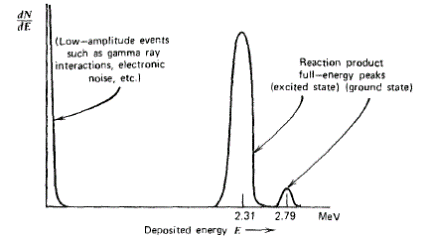
\includegraphics[scale=0.65]{ch11/image1}
	\captionof{figure}{Spectre idéal pour un compteur au $BF_5$. Si il a de grandes dimensions, 
	les produits de la réaction sont créés loin des parois et déposent toutes leur énergie $Q$ dans 
	le gaz du compteur}
	\end{wrapfigure}
On utilise généralement du $BF_3$ ou de l'$^3$H gazeux car il n'existe pas de gaz stable à 
base de lithium. Ces deux gaz présente une bonne discrimination aux $\gamma$. Lorsque les
$\gamma$ interagissent avec les parois, ils produisent des électrons. Ces-derniers ne perdent
que peu d'énergie dans le gaz, les impulsions produites sont bien plus courtes que celles des 
neutrons : discriminable. Cependant la résolution temporelle est mauvaise car c'est un produit
de réaction qu'il faut tout d'abord amorcer. Le $BF_3$ est très toxique et électronégatif ce qui
fait une chambre à gaz médiocre. Les détecteurs à base de $^3$He sont bien meilleurs mais
sont \textbf{très} chers.\\

\subsubsection{Effet de paroi pour un $BF_3$}
	\begin{wrapfigure}[4]{r}{3cm}
	\vspace{-17mm}
	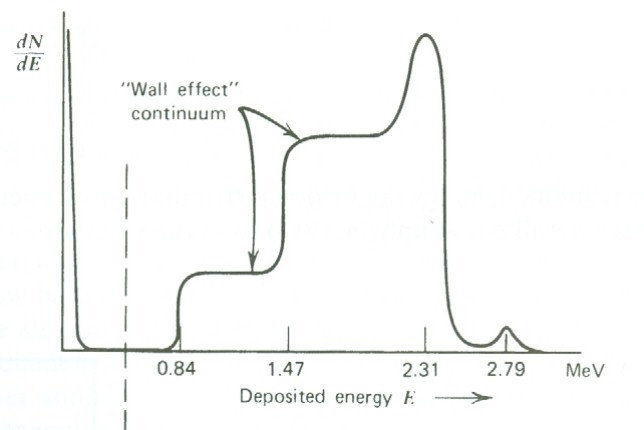
\includegraphics[scale=0.2]{ch11/image2}
	\captionof{figure}{ }
	\end{wrapfigure}
Si la taille du détecteur n'est pas beaucoup plus grande que le range du $\alpha$ et du Li, il y
aura des interactions avec les parois du détecteur. Une partie de l'énergie disponible est alors
déposée dans les parois ce qui modifie le spectre par \textit{effet de paroi}.
\begin{enumerate}
\item Si le $\alpha$ et Li sont émis dans des direction opposée et que le $\alpha$ interagit avec
une paroi, le LI dépose toute son énergie dans le gaz. L'énergie déposée varie de $E_{Li}$ à 
$E_{Li}+E_\alpha$.
\item Si inversement le Li interagit avec une paroi, le $\alpha$ dépose toute son énergie dans le
gaz et l'énergie déposée varie entre $E_\alpha$ et $E_\alpha+E_{Li}$.
\item Si le $\alpha$ et le Li sont créés "loin" des parois, l'échappement n'est pas possible et 
on a un pic d'absorption en $E_\alpha+E_{Li}$.
\end{enumerate}
La combinaison de ces différent processus donne le spectre suivant
\begin{center}
	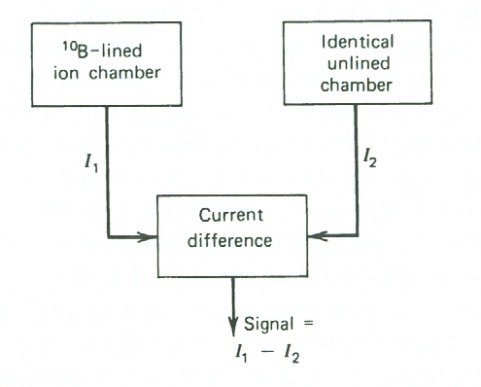
\includegraphics[scale=0.6]{ch11/image3}
	\captionof{figure}{ }
\end{center}
Le compteur du $^3$He fonctionne exactement sur le même principe mais comme $Z$ est plus faible,l'effet de paroi est plus important à une taille et pression identique.
\newpage


\subsection{Scintillateurs neutrons}%sl16
On peut utiliser du Li dopé à l'Eu : LiI(EU). Lorsque le neutron réagit avec le lithium cela produit
du tritium et des $\alpha$ qui interagissent "classiquement" avec le scintillateur. En choisissant
des cristaux de grande taille on peut éviter l'effet de paroi et avoir un pic d'absorption total.
Le désavantage est que le cristal scintillant est sensible au $\gamma$ qui vont déposer toute leur
énergie, rendant la discrimination peu efficace.


\subsection{Détecteurs neutrons basés sur la fission}%sl18
Les réaction de fission convertissent les neutrons lents en produits de réaction ionisants que l'on
détecte conventionnellement : une énergie de 200 MeV est disponible et 160 MeV est communiquée aux
fragments de fission. Mais comme on ne peut pas mettre de matières fissiles dans un gaz, il faut 
recouvrir l'enceinte interne d'un détecteur à gaz de matière fissile. Il ne faut cependant pas 
mettre une trop grosse épaisseur car même si l'efficacité de détection augmente, l'absorption 
énergétique dans le dépôt lui-même augmente ce qui cause des distorsions du spectre.


\subsection{Détecteurs neutrons pour les réacteurs nucléaires}%sl23
Il faut cette fois-ci détecter les neutrons lents. On utilise souvent es détecteurs à gaz afin
de les discriminer des $\gamma$ mais aussi pour leur stabilité à long terme et leur résistance aux
dégâts radiatifs. Dans tous les cas on n'utilise jamais de SC car ceux-ci sont très sensibles aux
radiations.\\

Il existe deux catégories de détecteur de neutrons en fonction du flux à mesurer

\begin{description}
\item[Out-of-core] en dehors du cœur des PWR. 
\item[In-core] Dans le cœur des BWR et des PWR. 
\end{description}\ 

\subsubsection{Détecteur out-of-core}
On peut utiliser les détecteurs à gaz comme détecteur \textit{out-of-core}. Le mode impulsion étant
limité à $10^7$ événements par seconde ce qui pose problème pour des flux plus élevé. Il faut alors
utiliser le mode courant mais il n'est plus possible de discriminer les $\gamma$. Deux possibilités
	\begin{enumerate}
	\item Utilisation du mode fluctuation : permet la discrimination
	\item Chambre d'ionisation compensée
	\end{enumerate}\ 


	\begin{wrapfigure}[7]{r}{3cm}
	\vspace{-5mm}
	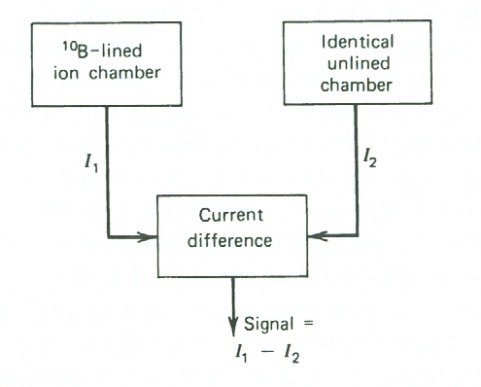
\includegraphics[scale=0.3]{ch11/image4}
	\captionof{figure}{ }
	\end{wrapfigure}
	
La chambre d'ionisation est une chambre ionisation classique où \textbf{une des} parois intérieures
est recouverte de Bore fonctionnant en mode courant. Le courant mesuré $I_1$ est alors la somme 
des courants dû aux interactions des neutrons dans le bore et des $\gamma$ dans les parois et le 
gaz. Sur l'\textbf{autre} paroi, on mesure $I_2$ dans une chambre normale : ce courant est dû aux
interactions des $\gamma$ dans les parois et le gaz. Comme $I_2$ n'est que sensible aux $\gamma$, la
différence des deux donne le courant dû aux neutrons.

\newpage
\subsubsection{Détecteurs in-core : chambre à fission}
	\begin{wrapfigure}[7]{l}{3cm}
	\vspace{-5mm}
	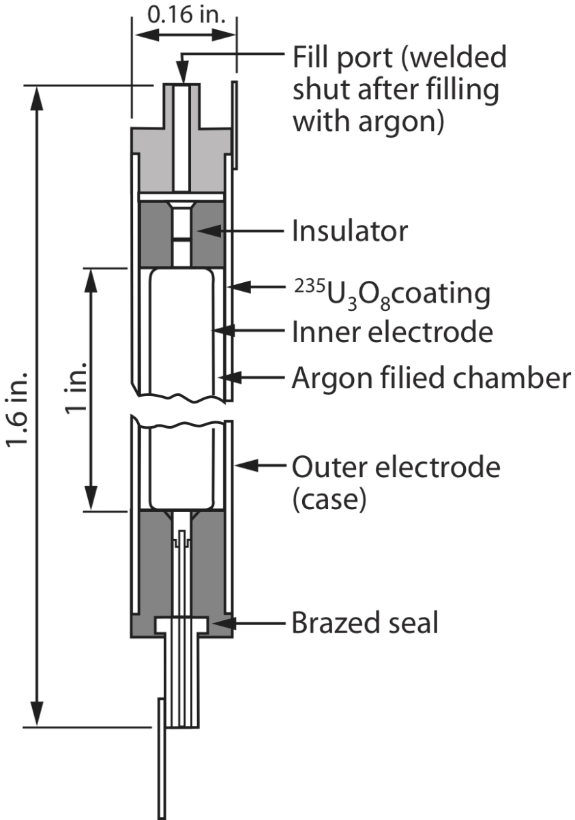
\includegraphics[scale=0.15]{ch11/image5}
	\captionof{figure}{ }
	\end{wrapfigure}
Dans les BWR on utilise généralement une chambre d'ionisation avec un dépôt $^{235}U$, en mode
courant. En utilisant de l'argon à haute pression, le range des produits de fission est inférieur
à la dimension de la chambre. Le problème est qu'il se consomme (50\% après un an). Pour compenser
ça, on utilise un mélange d'isotope fissile et fertile qui vont se convertir en matière fissile.\\
\ \\
\vspace{3mm}

On peut aussi utiliser des \textit{détecteurs auto-alimentés} comme détecteur in-core. Il s'agit
de détecteurs contenant un matériau avec une grande section efficace de capture électronique
impliquant un processus d'émission de $\beta$ ou de $\gamma$. En fonction de ce qui est émis
\begin{itemize}
\item[$\bullet$] Émission $\beta$ : mesure du courant directement et celui-ci $\propto$ taux de
capture des neutrons.
\item[$\bullet$] Émission $\gamma$ : interagissent par effet photoélectrique/\textsc{Compton}/création
de paires donnant lieu à des électrons secondaires et donc un courant.
\end{itemize}\ 

L'avantage de tels détecteurs est leur petite taille, faible coût et électronique simple. Par contre,
le courant de sortie est faible et il est obligatoire de l'utiliser en mode courant. La sortie 
temporelle est donc lente. Pour l'émission $\beta$, on choisira un matériau avec une section efficace
de capture électronique ni trop faible (faible sensibilité), ni trop élevée (auto-absorption). Pour
les $\gamma$, on peut utiliser du $^{59}$Co.

\section{Méthodes de détection des neutrons rapides}
\subsection{Détection après modération}%sl33
	\begin{wrapfigure}[8]{l}{6cm}
	\vspace{-5mm}
	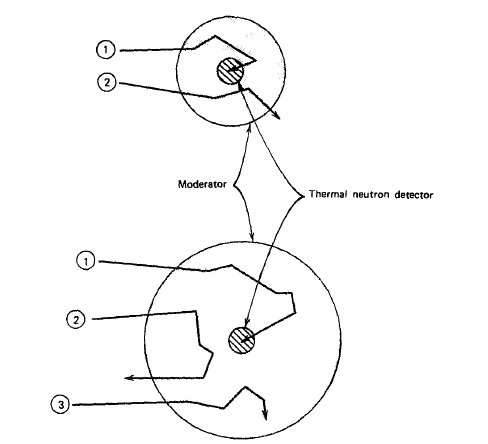
\includegraphics[scale=0.4]{ch11/image6}
	\captionof{figure}{ }
	\end{wrapfigure}

Il faut entourer le détecteur d'un modérateur (1-10cm) d'un matériau contenant de l'hydrogène de sorte
à ce que les neutrons perdent une importante part de leur énergie cinétique avant d'atteindre un
détecteur sensible aux neutrons lents. L'épaisseur du modérateur doit donc dépendre de l'énergie
du flux de neutrons.
\begin{itemize}
\item[$\bullet$] \textit{Neutrons de faible énergie} (keV). Si modérateur\ trop épais, perte de signal.

\item[$\bullet$] \textit{Neutrons d'énergie élevée} (MeV). Si trop mince : pas assez modéré et 
pas détectés.
\item[$\bullet$] \textit{Neutrons d'énergie > 10} MeV. La réponse du détecteur chute.
\end{itemize}\ \\

Il y a donc trois cas possibles, représentés ci-contre
\begin{enumerate}
\item Neutron modéré et détecté.
\item Neutron partiellement modéré s'échappant sans atteindre le détecteur (il passe à travers, 
c'est ce qui se passe sur le détecteur est trop petit).
\item Neutron capturé par le modérateur (et donc non détecté).
\end{enumerate}\ 

Il faut donc trouver un compromis en fonction de l'énergie du neutron.

\newpage
\subsection{Sphère de Bonner}
	\begin{wrapfigure}[8]{l}{4.5cm}
	\vspace{-5mm}
	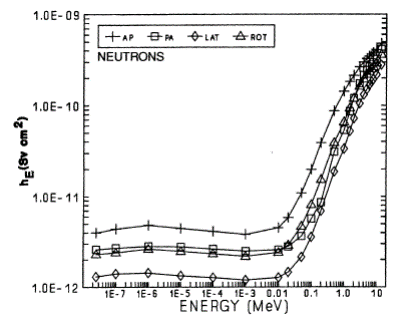
\includegraphics[scale=0.4]{ch11/image7}
	\captionof{figure}{ }
	\end{wrapfigure}
Il s'agit d'un détecteur sphérique constitué d'un petit scintillateur LiI placé au centre d'une 
sphère modératrice de polyéthylène. La réponse est très variable en fonction de la taille du 
détecteur. On a remarqué la courbe en réponse pour un diamètre de 12 pouces a une forme similaire
à celle de la dose équivalente à un milieu biologique\footnote{Il s'agit d'une pure coïncidence 
mais très utile}. Le détecteur aura donc une grande efficacité pour les neutrons avec une grande
importance biologique et faible pour les autres, la pondération est automatiquement inclue.\\


\subsection{Compteur long}
	\begin{wrapfigure}[10]{r}{5.5cm}
	\vspace{-5mm}
	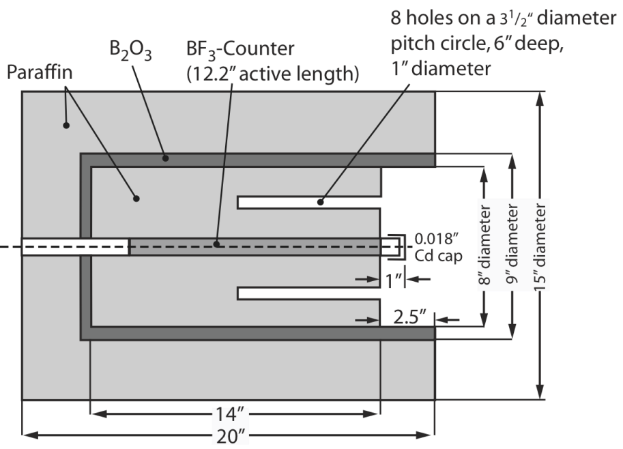
\includegraphics[scale=0.35]{ch11/image8}
	\captionof{figure}{ }
	\end{wrapfigure}
L'efficacité de la détection est indépendante de l'énergie des neutrons pour une géométrie donnée.
Sur la figure ci-contre, il est uniquement sensible aux neutrons incidents sur la face de droite.
Les neutrons parallèles à l'axe parcourent une certaine distance avant la modération (plus ou moins
grande en fonction de l'énergie). Si le tube est assez long, le neutron sera à la fin détecté. On 
ne peut pas discriminer les neutrons lents des rapides mais au moins on détecte les deux. Les 
neutrons non parallèles sont modérer dans la paroi annulaire de paraffine puis capturés dans le 
B$_2$O$_3$ : non comptés.

\subsection{Détection des neutrons rapides ($E>10$ MeV)}
	\begin{wrapfigure}[6]{l}{4cm}
	\vspace{-7mm}
	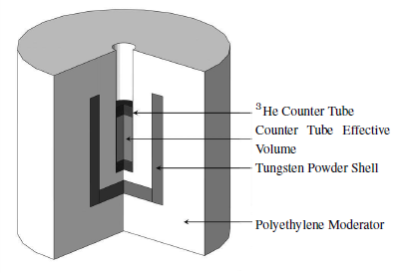
\includegraphics[scale=0.35]{ch11/image9}
	\captionof{figure}{ }
	\end{wrapfigure}
Les neutrons rapides ont une énergie très élevé. En rajoutant une couche de métal lourd ($W$), 
celui-ci ne modère pas mais présente des réaction $(n,2n)$ multipliant le nombre de neutrons et
augmentant la fonction de réponse jusqu'au GeV. On "compense" en quelque sorte les neutrons perdus,
passés à travers le détecteur à cause de leur grande énergie. Ca peut sembler artificiel, mais ça
marche bien.

\subsection{Détecteur neutrons avec diodes}
	\begin{wrapfigure}[9]{l}{9cm}
	\vspace{-5mm}
	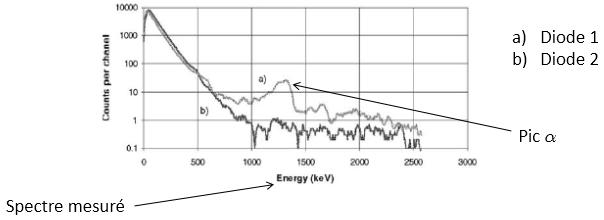
\includegraphics[scale=0.55]{ch11/image10}
	\captionof{figure}{ }
	\end{wrapfigure}
On peut faire un détecteur de neutrons qui se base sur l'utilisation de deux diodes. Une première
(\textit{diode neutron}) recouverte d'un matériau organique enrichi au $^{10}$B sensible aux 
neutrons et aux $\gamma$. Une seconde (\textit{diode} $\gamma$) nue de sorte à être peu sensible
aux $\gamma$ et sensible aux neutrons. On place ensuite les deux diodes côtés à côté, 
perpendiculairement aux rayonnements ionisants. Les neutrons thermiques interagissent avec la 
première diode de deux façons
\begin{enumerate}
\item $H(n,n)p \to $ émission de protons
\item $^{10}$B(n,$\alpha$)$^7$Li $\to$ émission de $\alpha$
\end{enumerate}\ 

La différence entre les deux diode permet de discriminer la composante due aux $\gamma$ de celle
due aux neutrons. En utilisant une taille importante pour la couverture plastique, on peut 
modérer de façon importante des neutrons de hautes énergie pour les étudier. La quantité de $^{10}$B
est choisie de manière à obtenir une réponse aux neutrons thermiques égales à celle aux neutrons
rapides. Comme précédemment, pour les très haute énergie ($E >$ 10 MeV), on ajoute une couche
de Pb pour avoir des réactions $(n,2n)$. On peut également faire un système à 3-4 diodes avec
différents recouvrements pour améliorer la précision d'une plage d'énergie importante. Ceci forme
alors un détecteur multi-éléments (détecteur Saphydose).


\subsection{Détection basée sur les réactions des neutrons rapides et spectrométrie neutronique}%sl47
Le problème des détecteurs basés sur la modération est qu'ils ne donnent aucune information sur 
l'énergie des neutrons et le processus de détection est lent (comme il faut d'abord les 
thermaliser). Pour résoudre le problème, on peut directement utiliser des réactions nucléaires pour
des neutrons rapides qui induisent des produits de réactions chargés qui eux peuvent être détectés. \\

L'énergie cinétique du produit de réaction vaut $Q$ + l'énergie cinétique du neutron incident. En
considérant que l'énergie du neutron incident est supérieur à une certaine fraction de $Q$,on obtient
l'énergie du neutron incident. Le processus de détection est donc rapide, mais son efficacité est
faible (sections efficaces faibles).\\

Deux familles de tels réacteurs existent
\begin{enumerate}
\item Utilisation des réactions $^6$Li($n,\alpha$) ou $^3$He($n,p)$ : idem aux détecteurs vus 
précédemment (l'énergie du $\alpha$ ou du proton doit être précisément mesurée).
\item Utilisation de la réaction de diffusion élastique ($\equiv Q=0$) en mesurant l'énergie de recul
du noyau impliqué dans la réaction neutron-noyau.
\end{enumerate}

\subsubsection{Détecteurs basés sur la diffusion élastique}
Pour maximiser le transfert d'énergie, on utilise des éléments légers. L'hydrogène est le plus 
populaire, on mesure alors un proton de recul ; \textit{détecteurs à proton de recul}. Comme par
 définition de la diffusion élastique $Q=0$, l'énergie du proton de recul peut être égale à celle
 du neutron incident.

\subsubsection{Scintillateurs organiques pour la détection des neutrons}
	\begin{wrapfigure}[11]{l}{7cm}
	\vspace{-5mm}
	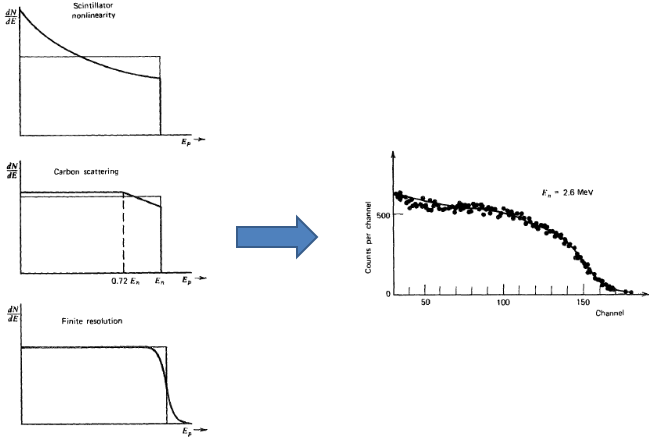
\includegraphics[scale=0.4]{ch11/image12}
	\captionof{figure}{ }
	\end{wrapfigure}
Les scintillateurs organiques contiennent de l'hydrogène : le stilbène possède une bonne 
discrimination aux $\gamma$. En première approximation, toutes les énergies cédée au proton sont
équiprobables (en réalité, $T_C = E.\cos^2\theta_r$). Le spectre en énergie mesuré est considéré
rectangulaire. Il y a cependant des écarts par rapport à un spectre rectangulaire (non-linéairité, 
effets de paroi, diffusions multiples, résolution du détecteur, diffusion avec le carbone
du scintillateur, \dots). Tous ces effets font donc que l'on s'éloigne de la forme rectangulaire.

\newpage

\subsection{Compteurs proportionnels pour la détection des neutrons }
Ceux-ci contiennent de l'hydrogène ou un gaz riche en ce-dernier comme du méthane. Comme un gaz a une
faible densité, l'efficacité est faible et l'effet de paroi est important. La pureté du gaz est
très importante, les impuretés peuvent causer des distorsions importantes : son utilisation est
moins pratique que celle des scintillateurs.


\subsubsection{Télescope à proton de recul}
	\begin{wrapfigure}[14]{l}{7.5cm}
	\vspace{-4mm}
	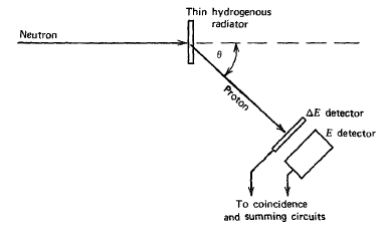
\includegraphics[scale=0.75]{ch11/image13}
	\captionof{figure}{ }
	\end{wrapfigure}
On considère un matériau riche en hydrogène. En mettant le détecteur à un angle précis et en mesurant
précisément l'énergieonpeut retrouver l'énergie du neutron. Nous avons des neutrons incidents
monoénergétique qui diffusent dans un film mince (inférieur au range des protons) mais riche en 
hydrogène. Comme $T_C=E.\cos^2\theta_r$, on peut obtenir l'énergie précise du proton pour un angle
donné, donnant un pic en énergie. Le problème est que l'émission est isotrope, ne sélectionner qu'un
angle donne une efficacité extrêmement faible (un coup pour $10^5$ neutrons), il est donc nécessaire
d'avoir un flux important pour avoir un résultat convaincant.

%\section{Méthodes de détection des neutrons lents}  ==> ????



\vspace{4cm}
\begin{center}

\includegraphics[scale=0.2]{ch11/fin}
\end{center}